%!TEX TS-program = xelatex
\documentclass[]{friggeri-cv}
\addbibresource{bibliography.bib}

\usepackage{graphicx}

\begin{document}
\header{Guillaume}{Gremillet}
       {\'Etudiant en informatique recherche stage assistant ingénieur (10-17 semaines)}


% In the aside, each new line forces a line break
\begin{aside}
    \centerline{\frame{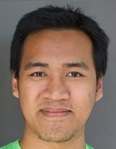
\includegraphics[width=3cm]{gremillg.jpg}}}~
    \section{Contact}
        19, Rue du Tour de l'Eau
        38400, Saint-Martin-d'Hères
        France
        ~
        10, Rue Blanche
        75009, Paris
        France
        ~
        \href{mailto:gui.gremi@gmail.com}{gui.gremi@gmail.com}
        06 71 09 81 48
    \section{Langues}
        Anglais (B2/C1)
        Espagnol (B1/B2)
    \section{Programmation}
        \textbf{Web}
        (Html/Css, Php, Javascript)
        \textbf{Dev}
        (C, Java, Ada, Python)
        \textbf{Mobile}
        (Ionic)
\end{aside}
    Impliqué dans tout ce que j’entreprends, je suis ouvert d’esprit, flexible et toujours prêt à aider. J’aime le travail bien fait tout en sachant me concentrer sur les aspects fonctionnels. Je me définis comme rationnel, pragmatique et sais m’amuser quand il le faut.

\section{\'Etudes}
\begin{entrylist}
    \entry
        {2015-2018}
        {\'Elève ingénieur Ensimag {\normalfont Ingénierie des Systèmes d'Information}}
        {Ensimag}
        {Bases de données et programmation ; système et algorithmique ; logique et réseaux ; projet de génie logiciel ; sciences humaines, économiques, du management et de l’entreprise}
    \entry
        {2013-2015}
        {Classes préparatoires PTSI/PT*}
        {Lycée Chaptal Paris}
        {Classe étoilée : Physique Technologies et Sciences Industrielles}
    \entry
        {2013}
        {Baccalauréat scientifique mention Très Bien}
        {Lycée Chaptal Paris}
        {Options Latin ; sciences industrielles ; histoire-géographie}
\end{entrylist}

\section{Expériences}
\begin{entrylist}
    \entry
        {\'Eté 2016}
        {Stagiaire}
        {Galway Community Circus, Irlande}
        {Organisation informatique, aide à la conception du site web, organisation d'un système de gestion de fichiers}
    \entry
        {2016-2017}
        {Responsable foyer/cafétéria}
        {Cercle des elèves Ensimag}
        {Développement d'applications web et mobiles ; logistique ; gestion de budget ; gestion d’équipe}
    \entry
        {Avril 2015}
        {Organisateur d'un voyage de classe}
        {Délégué de classe - Lycée Chaptal Paris}
        {Organisation d’un voyage scolaire d’une semaine à Berlin en tant que délégué de classe: Gestion de budget ; planning ; contact sur place ; coordination de groupe}
    \entry
        {Juillet 2013}
        {Accompagnateur de séjour / Traducteur}
        {Association MO.O.V.E.}
        {Accompagnement d’un groupe de jeune en insertion professionnelle. Traduction anglais/français et participation aux activités circassiennes quotidiennes}
\end{entrylist}

\section{Intérêts}
\begin{entrylist}
    \entry
        {Musique}
        {Luth baroque}
        {Répertoire baroque}
        {Conservatoire d'arrondissement CMA9 puis Conservatoire à Rayonnement Intercommunal de Bernay}
    \entry
        {Sport}
        {Aïkido (3e Kyu), Karaté, Escrime, Tir à l'arc}
        {Sports individuels de travail sur soi}
        {EJUG, Taïkidojo, Aïkido Club Parisien ; École Parisienne de Karaté ; Club d’Escrime de Paris Tour d’Auvergne}    
    \entry
        {Associatif}
        {Cercle Ensimag}
        {Bureau des élèves Ensimag}
        {Responsable foyer/cafétéria \& Membre du staff événementiel : Travail d’équipe, planification, développement d’outils de gestion}
\end{entrylist}

\end{document}
